\documentclass[tikz,border=7pt]{standalone}
\begin{document}
  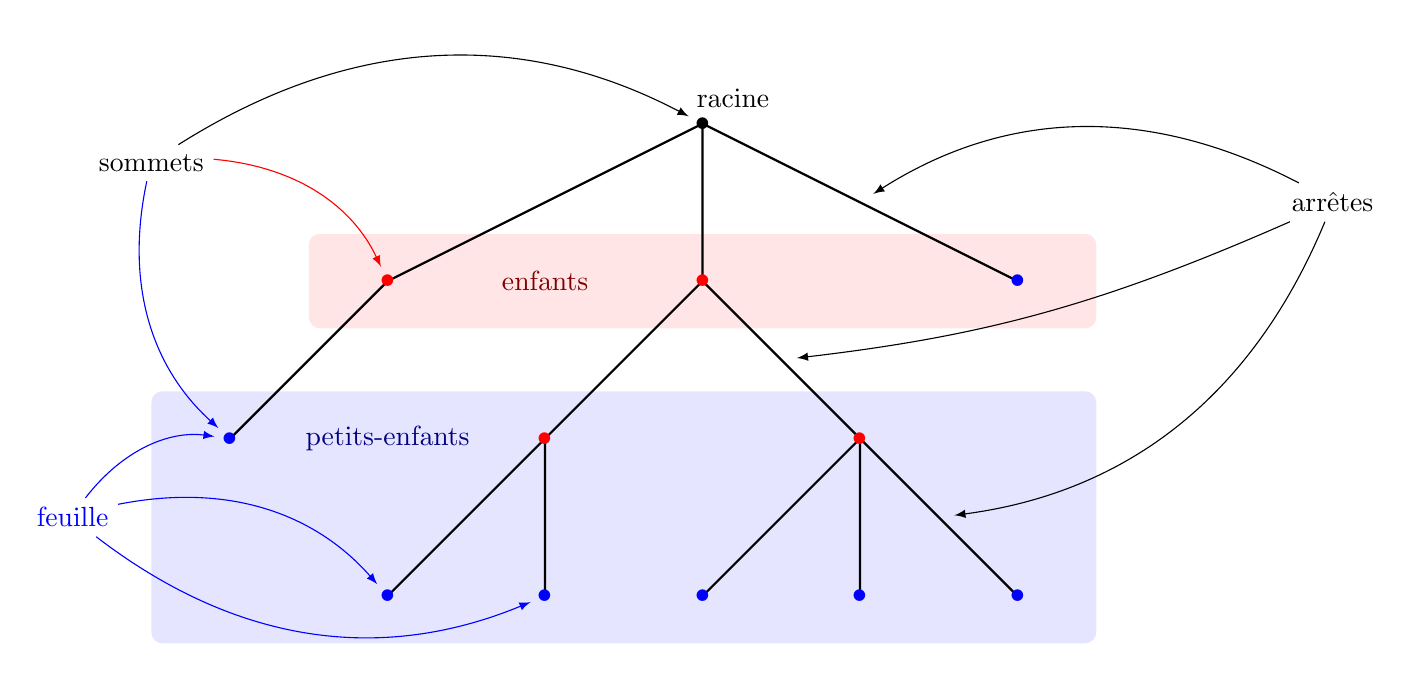
\begin{tikzpicture}[scale=2]
    % define points
    \path
      (0,0) coordinate(R)
      +(-2,-1) coordinate(V1)
      +(0,-1) coordinate(V2)
      +(2,-1) coordinate(V3)
      (V1)
      +(-1,-1) coordinate(V11)
      (V2)
      +(-1,-1) coordinate(V21)
      +(1,-1) coordinate(V22)
      (V21)
      +(-1,-1) coordinate(V211)
      +(0,-1) coordinate(V212)
      (V22)
      +(-1,-1) coordinate(V221)
      +(0,-1) coordinate(V222)
      +(1,-1) coordinate(V223)
    ;
    % zones
    \fill[red!10, rounded corners]
      (-2.5,-.7) rectangle (2.5,-1.3)
      (-1,-1) node[red!50!black]{enfants}
    ;
    \fill[blue!10, rounded corners]
      (-3.5,-1.7) rectangle (2.5,-3.3)
      (-2,-2) node[blue!50!black]{petits-enfants}
    ;
    % draw lines
    \draw[thick]
      (R) -- (V1)
      (R) -- coordinate(E0-2) (V2)
      (R) -- coordinate(E0-3) (V3)
      (V1) -- (V11)
      (V2) -- (V21)
      (V2) -- coordinate(E2-22) (V22)
      (V21) -- (V211)
      (V21) -- (V212)
      (V22) -- (V221)
      (V22) -- (V222)
      (V22) -- coordinate(E22-223) (V223)
    ;
    % draw points
    \path[
      r/.style = {black},
      v/.style = {red},
      l/.style = {blue},
      f/.style = {purple}
    ]
    foreach \v/\t in {R/r,V1/v,V2/v,V3/l,V11/l,V21/v,V22/v,V211/l,V212/l,V221/l,V222/l,V223/l}{
      (\v) node[scale=4,\t]{.}
    };
    % labels
    \path
      (R) node[anchor=-140, inner sep=2mm]{racine}
    ;
    \path[-latex, shorten > = 2mm]
      (-3.5,-.25) node(S){sommets}
      (S) edge[bend left] (R)
      (S) edge[bend left, red] (V1)
      (S) edge[bend right, blue] (V11)
    ;
    \path[-latex, shorten > = 2mm, blue]
      (-4,-2.5) node(F){feuille}
      (F) edge[bend left, blue] (V11)
      (F) edge[bend left, blue] (V211)
      (F) edge[bend right, blue] (V212)
    ;
    \path[-latex, shorten > = 2mm]
      (4,-.5) node(E){arrêtes}
      % (E) edge[bend left] (E0-2)
      (E) edge[bend right] (E0-3)
      (E) edge[bend left=3mm] (E2-22)
      (E) edge[bend left] (E22-223)
    ;
  \end{tikzpicture}
\end{document}
